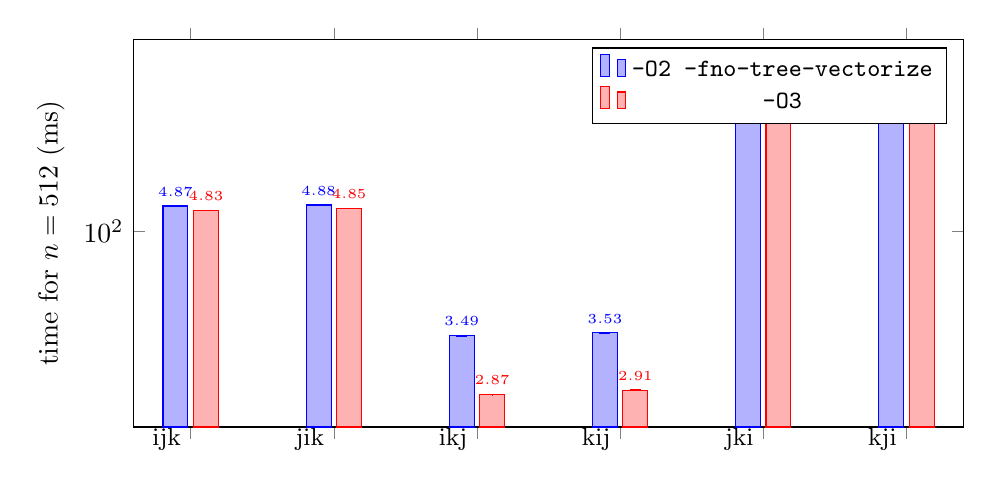
\begin{tikzpicture}
\begin{axis}[ybar, width=\textwidth, height=6.5cm, bar width=9pt, ymode=log, log origin=infty, symbolic x coords={ijk,jik,ikj,kij,jki,kji}, xtick=data, x tick label style={rotate=0, anchor=east, font=\small}, ylabel={time for $n=512$ (ms)}, enlarge x limits=0.08, legend style={font=\small, at={(0.98,0.98)}, anchor=north east}, nodes near coords, nodes near coords style={font=\tiny}, every node near coord/.append style={/pgf/number format/.cd, fixed, precision=2}]
\addplot+[error bars/.cd, y dir=both, y explicit] coordinates {(ijk,130.4100) +- (0,0.3500) (jik,131.8600) +- (0,0.2400) (ikj,32.9400) +- (0,0.1000) (kij,33.9600) +- (0,0.0350) (jki,534.4100) +- (0,0.3700) (kji,531.4200) +- (0,3.0550)};
\addlegendentry{\texttt{-O2 -fno-tree-vectorize}}
\addplot+[error bars/.cd, y dir=both, y explicit] coordinates {(ijk,124.7500) +- (0,0.0800) (jik,127.2700) +- (0,0.0850) (ikj,17.6500) +- (0,0.0350) (kij,18.4500) +- (0,0.0650) (jki,540.1000) +- (0,0.1200) (kji,536.3400) +- (0,0.1650)};
\addlegendentry{\texttt{-O3}}
\end{axis}
\end{tikzpicture}